Nesta seção, apresentamos os resultados da análise espectral do sinal, focando na comparação de diferentes filtros aplicados tanto a sinais de áudio quanto a imagens para remoção de ruído.

\subsection{Resultados da filtragem em sinal de áudio}
As figuras ~\ref{fig:audio_butterworth_spectrums} e ~\ref{fig:audio_elliptical_spectrums} mostram os espectros de frequências e as respostas em frequência dos filtros Butterworth e Elíptico em um áudio ruidoso.

\begin{figure}[H]
    \centering
    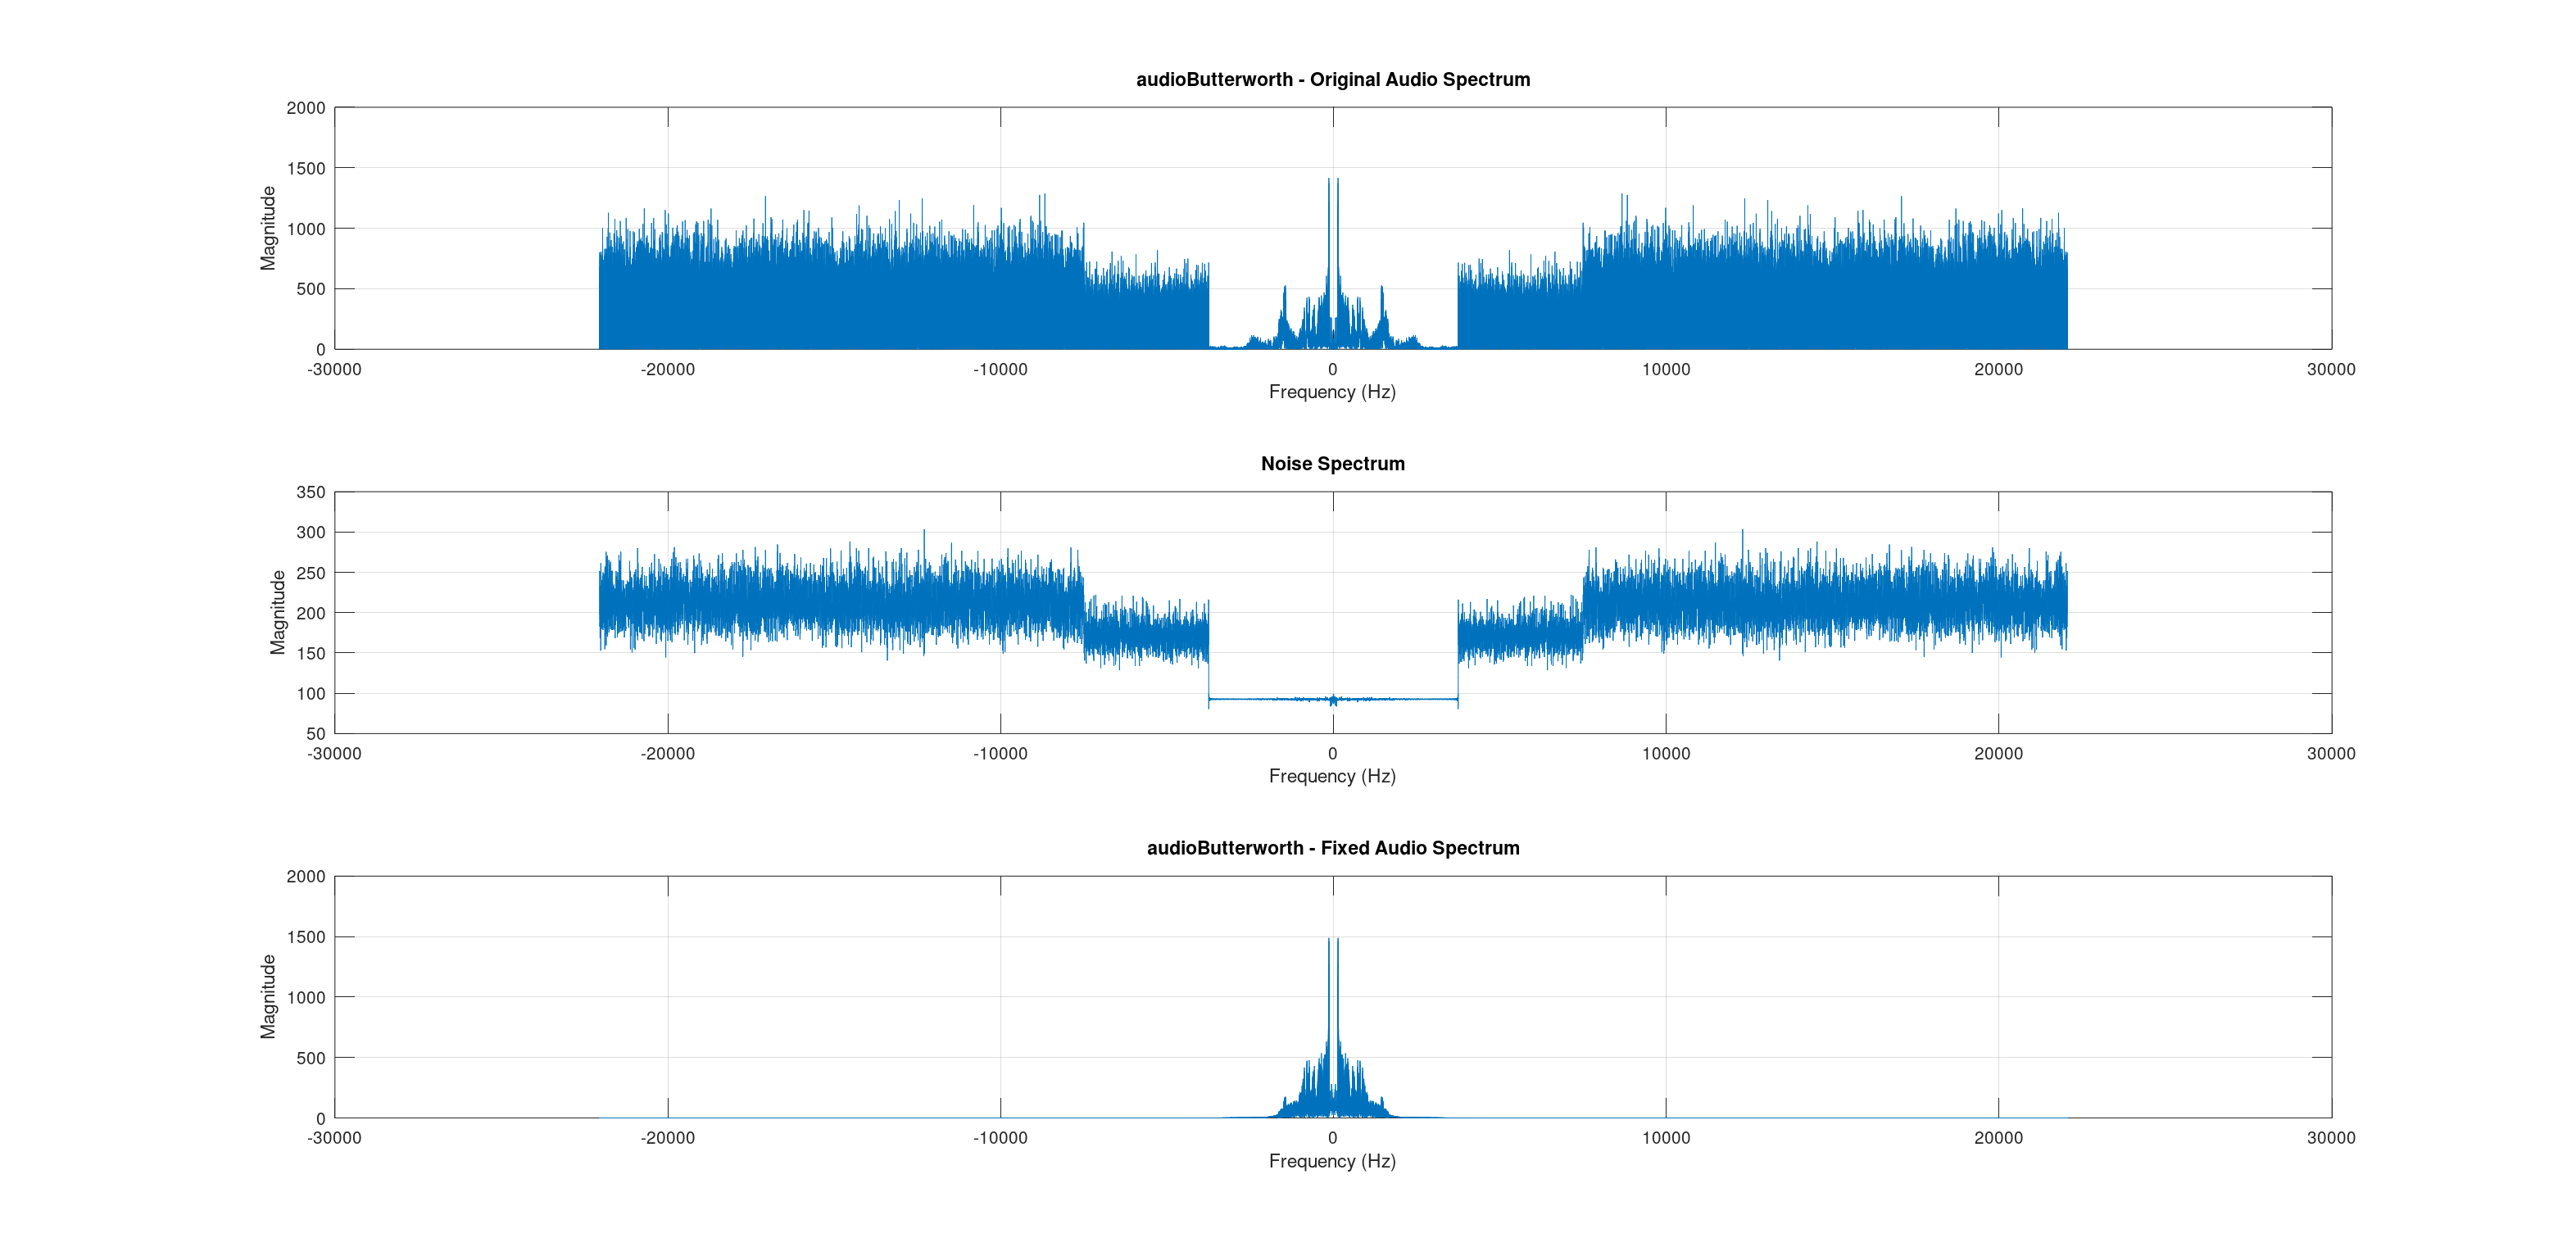
\includegraphics[width=1\linewidth]{03_results/assets/audio_butterworth_spectrums.png}
    \caption{Espectro de frequência do sinal de áudio antes e após a aplicação do filtro Butterworth.}
    \label{fig:audio_butterworth_spectrums}
\end{figure}

O filtro \textbf{Butterworth} é caracterizado por sua resposta suave e sem ondulação, proporcionando uma atenuação gradual das frequências fora da faixa desejada. Na figura \ref{fig:audio_butterworth_spectrums}, podemos observar como o filtro atua suavemente, permitindo que a faixa passante do sinal de áudio se mantenha praticamente intacta, enquanto o ruído de alta frequência é atenuado.

\begin{figure}[H]
    \centering
    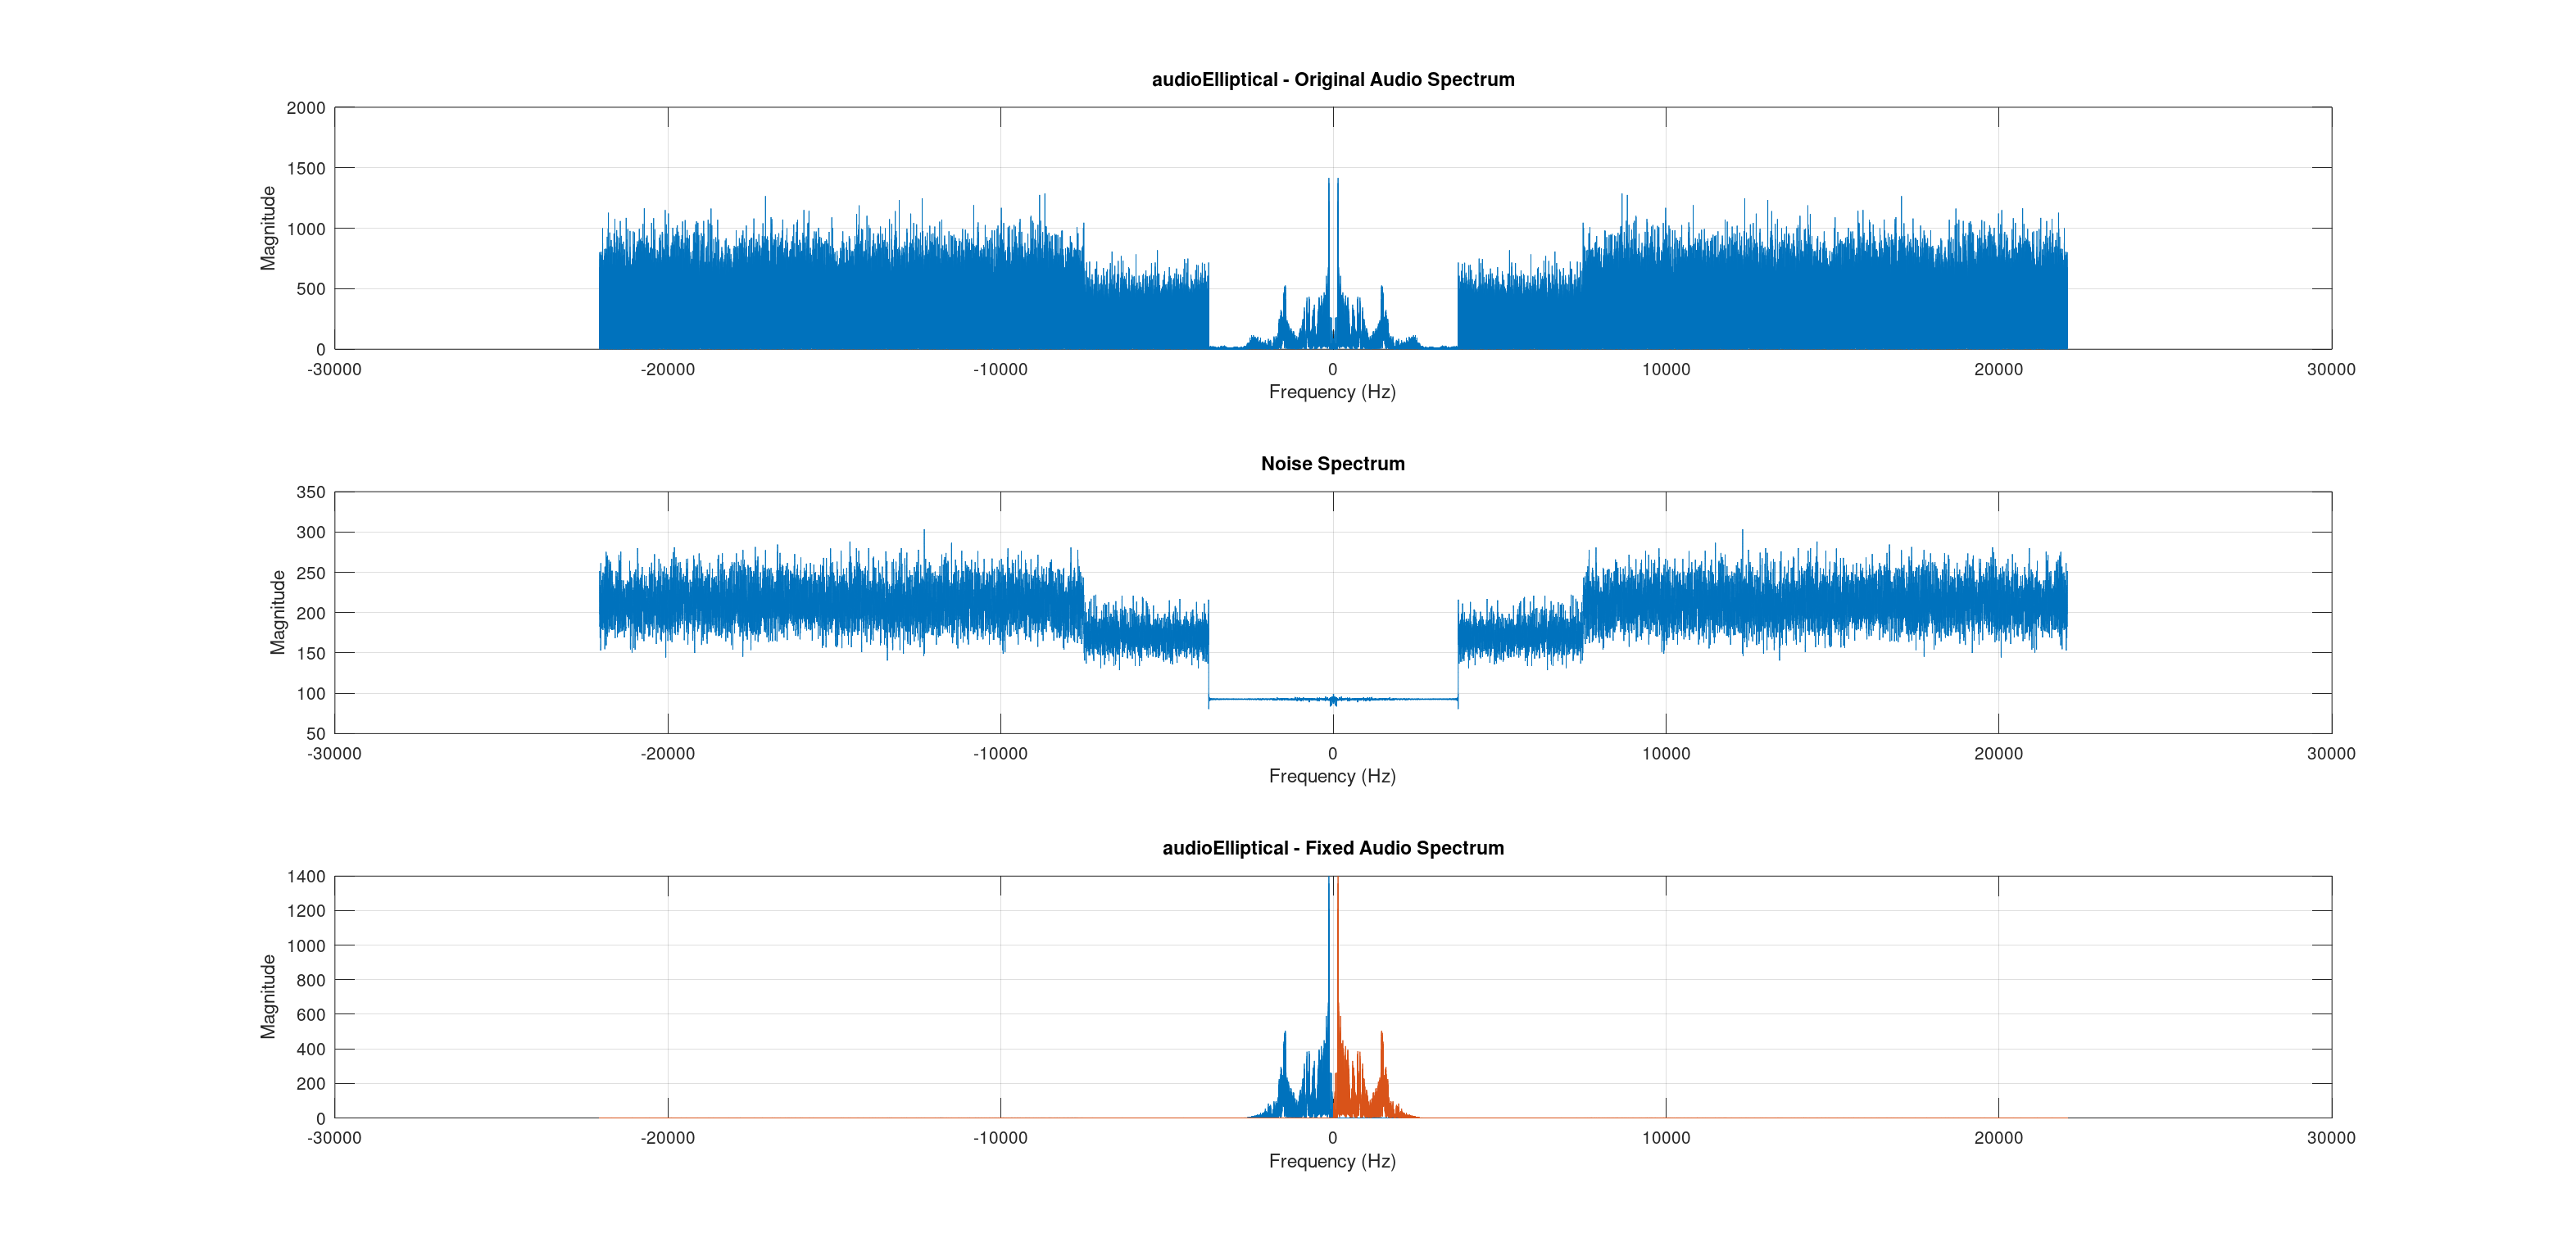
\includegraphics[width=1\linewidth]{03_results/assets/audio_elliptical_spectrums.png}
    \caption{Espectro de frequência do sinal de áudio antes e após a aplicação do filtro Elíptico.}
    \label{fig:audio_elliptical_spectrums}
\end{figure}

O filtro \textbf{Elíptico}, diferente do Butterworth, apresenta uma atenuação mais agressiva nas frequências fora da faixa passante. A principal característica desse filtro é a \textbf{ondulação} na resposta de magnitude, tanto na faixa passante quanto na faixa de rejeição. Isso permite uma filtragem mais eficiente, removendo frequências indesejadas de forma mais agressiva. No entanto, as oscilações na transição entre a faixa passante e a faixa de rejeição podem resultar em distorções perceptíveis, especialmente quando a integridade do sinal precisa ser preservada.

\subsection{Resultados da filtragem em Imagem Digital}
Como apresentado na Figura ~\ref{fig:image_original_plus_noise}, foi carregada uma imagem original 256x256 pixels, e aplicado um ruído senoidal na mesma.

\begin{figure}[H]
    \centering
    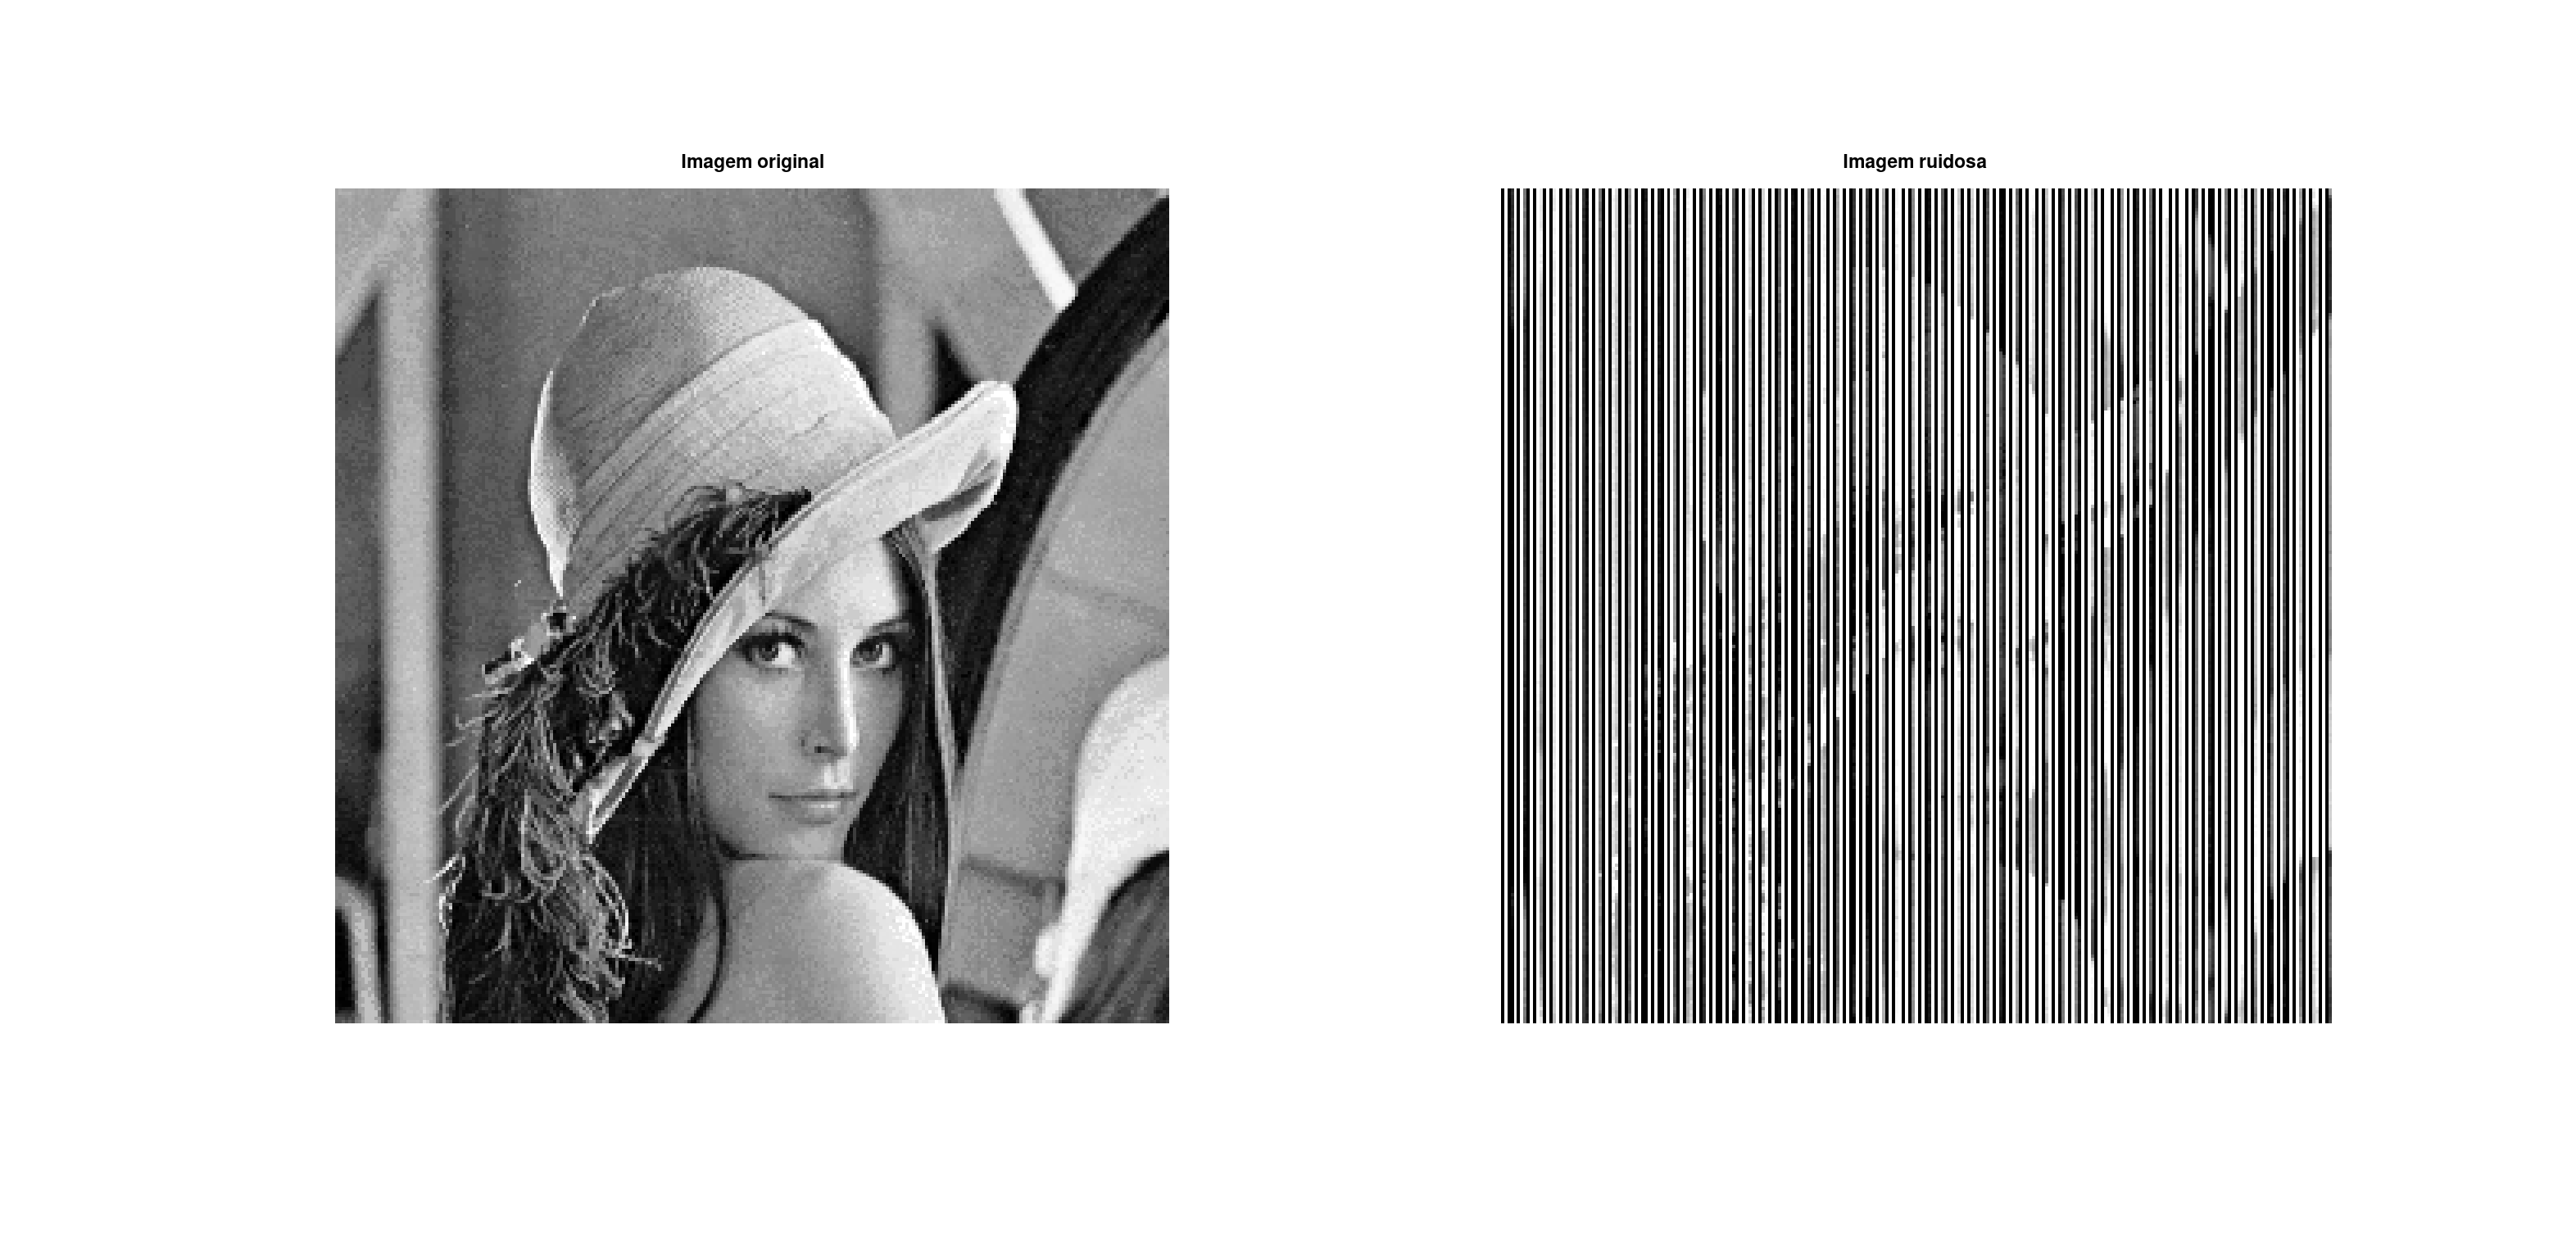
\includegraphics[width=1\linewidth]{03_results/assets/image_original_plus_noise.png}
    \caption{Imagem original e imagem ruidosa}
    \label{fig:image_original_plus_noise}
\end{figure}

Na figura \ref{fig:image_butterworth}, vemos a imagem filtrada com o filtro Butterworth em conjunto com o espectro do mesmo. Este filtro é eficaz na remoção de ruído de alta frequência sem afetar significativamente as bordas ou detalhes importantes da imagem. Ele suaviza as transições, mas mantém a maior parte da estrutura da imagem.

\begin{figure}[H]
    \centering
    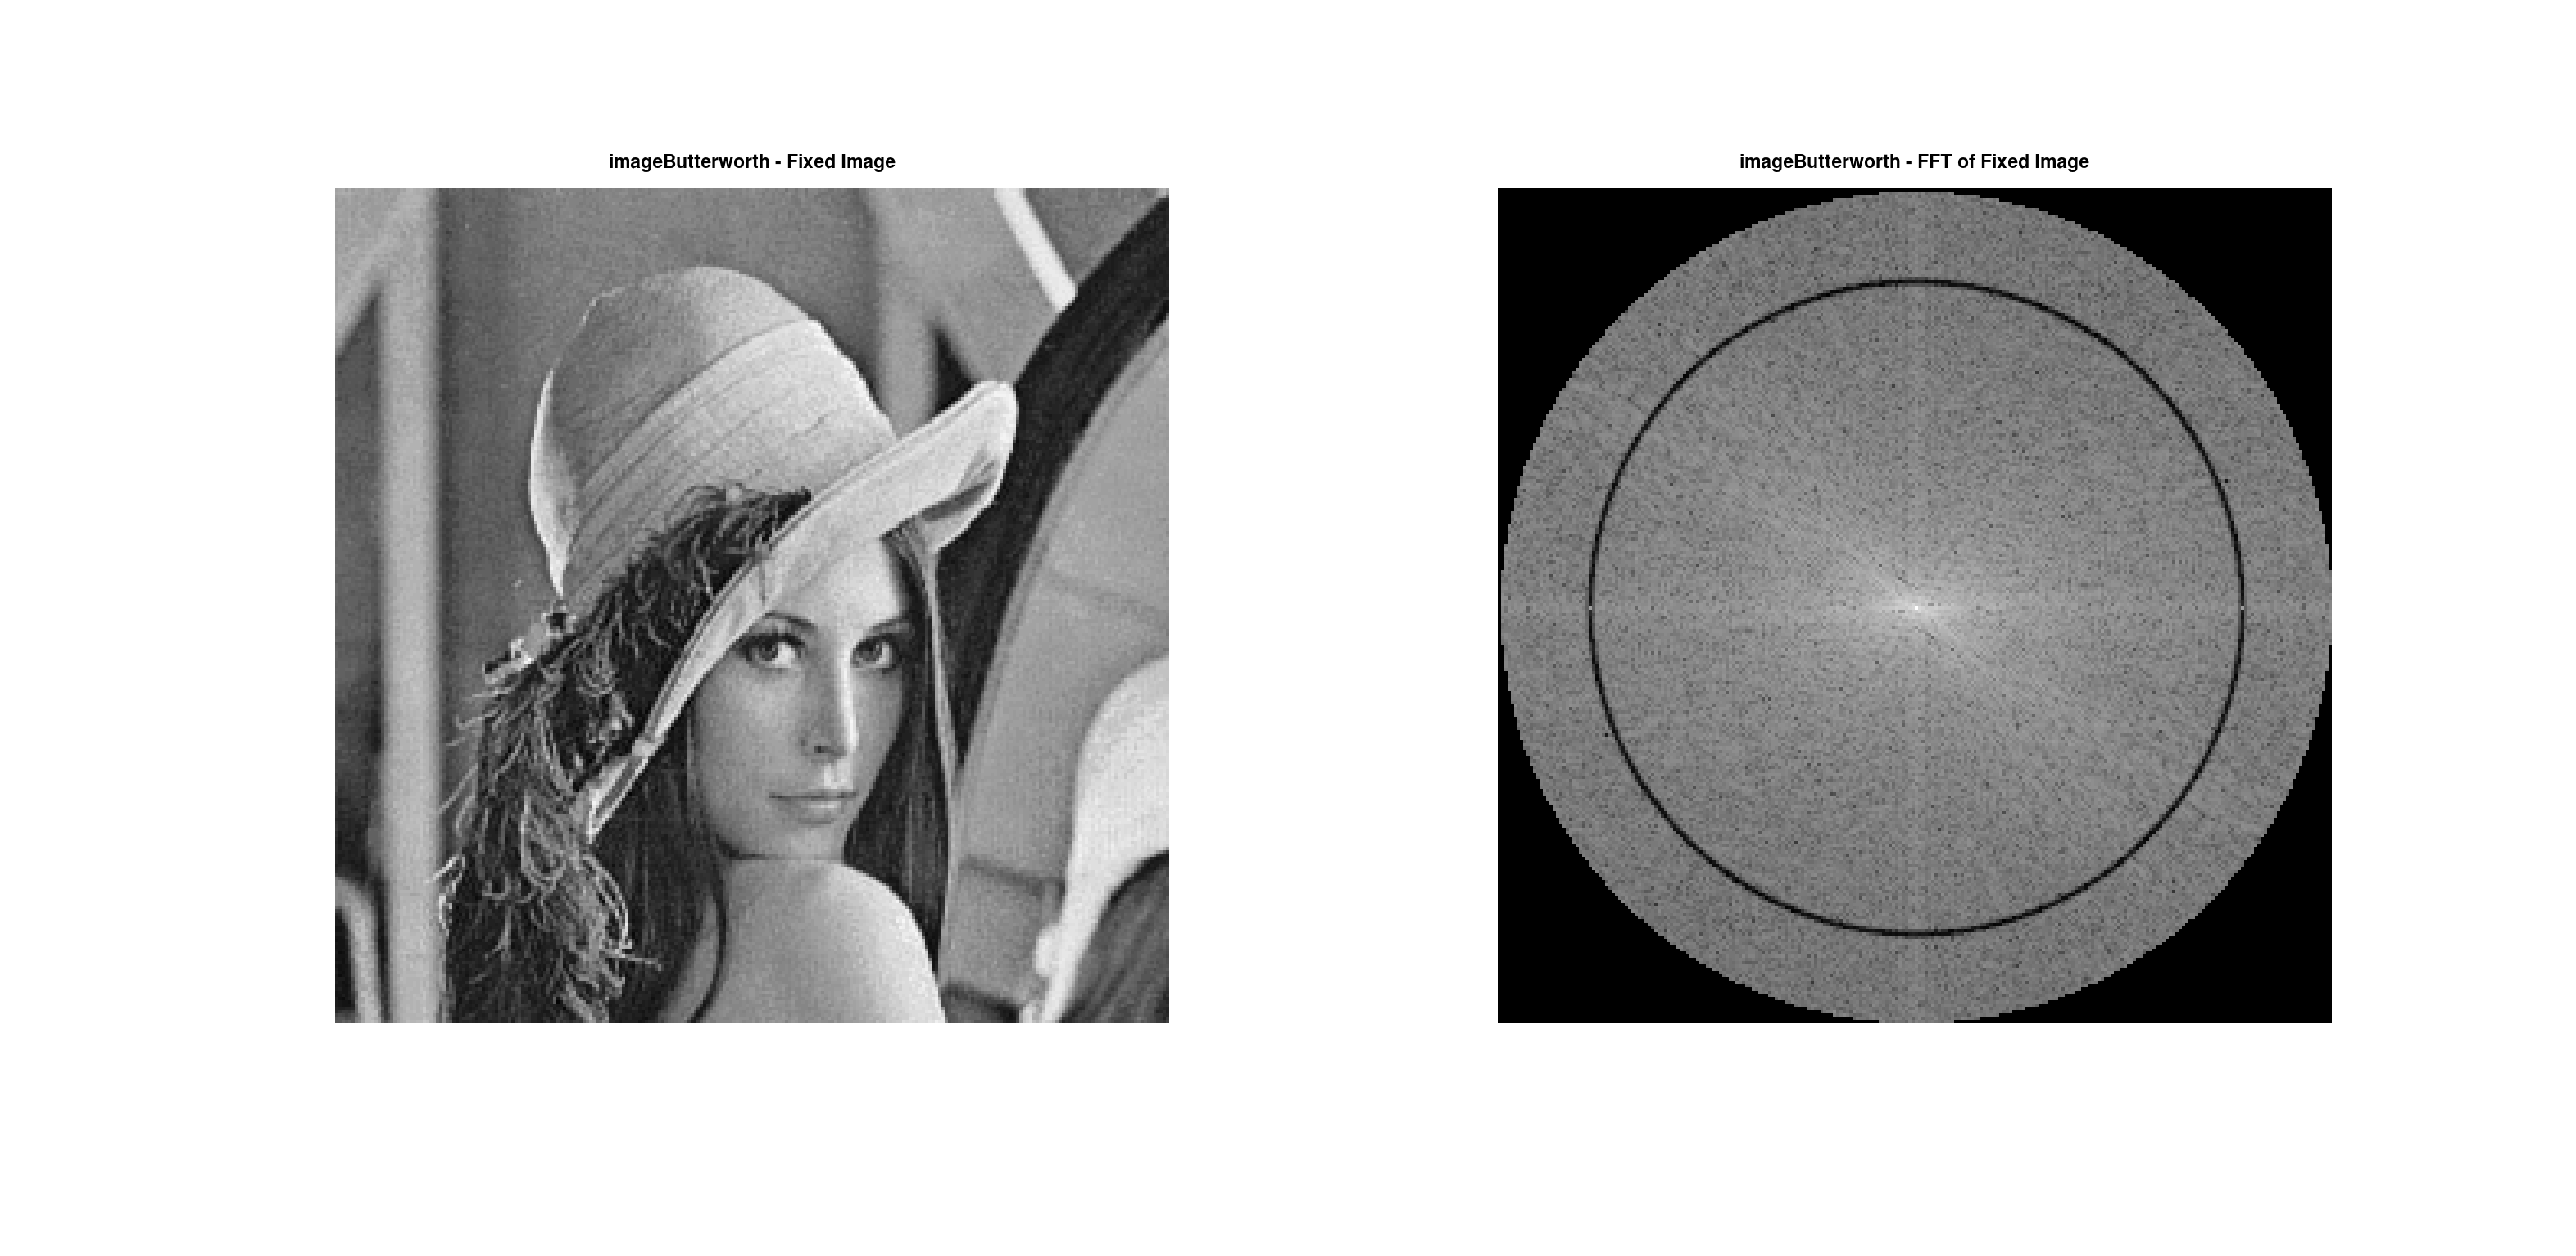
\includegraphics[width=1\linewidth]{03_results/assets/image_butterworth.png}
    \caption{Imagem filtrada e seu espectro com o filtro Butterworth.}
    \label{fig:image_butterworth}
\end{figure}

Enquanto que na figura \ref{fig:image_chebyshev} é mostrada a aplicação do filtro \textbf{Chebyshev}. Este filtro, sendo mais agressivo do que o Butterworth, apresenta uma resposta em frequência mais acentuada, permitindo uma remoção mais eficaz de ruídos em frequências específicas. No entanto, ele também pode introduzir distorções visíveis, especialmente em áreas com transições suaves, como as bordas da imagem. As oscilações na resposta de frequência podem resultar em artefatos indesejáveis, tornando-o uma escolha mais arriscada quando a preservação da qualidade visual é crítica.

\begin{figure}[H]
    \centering
    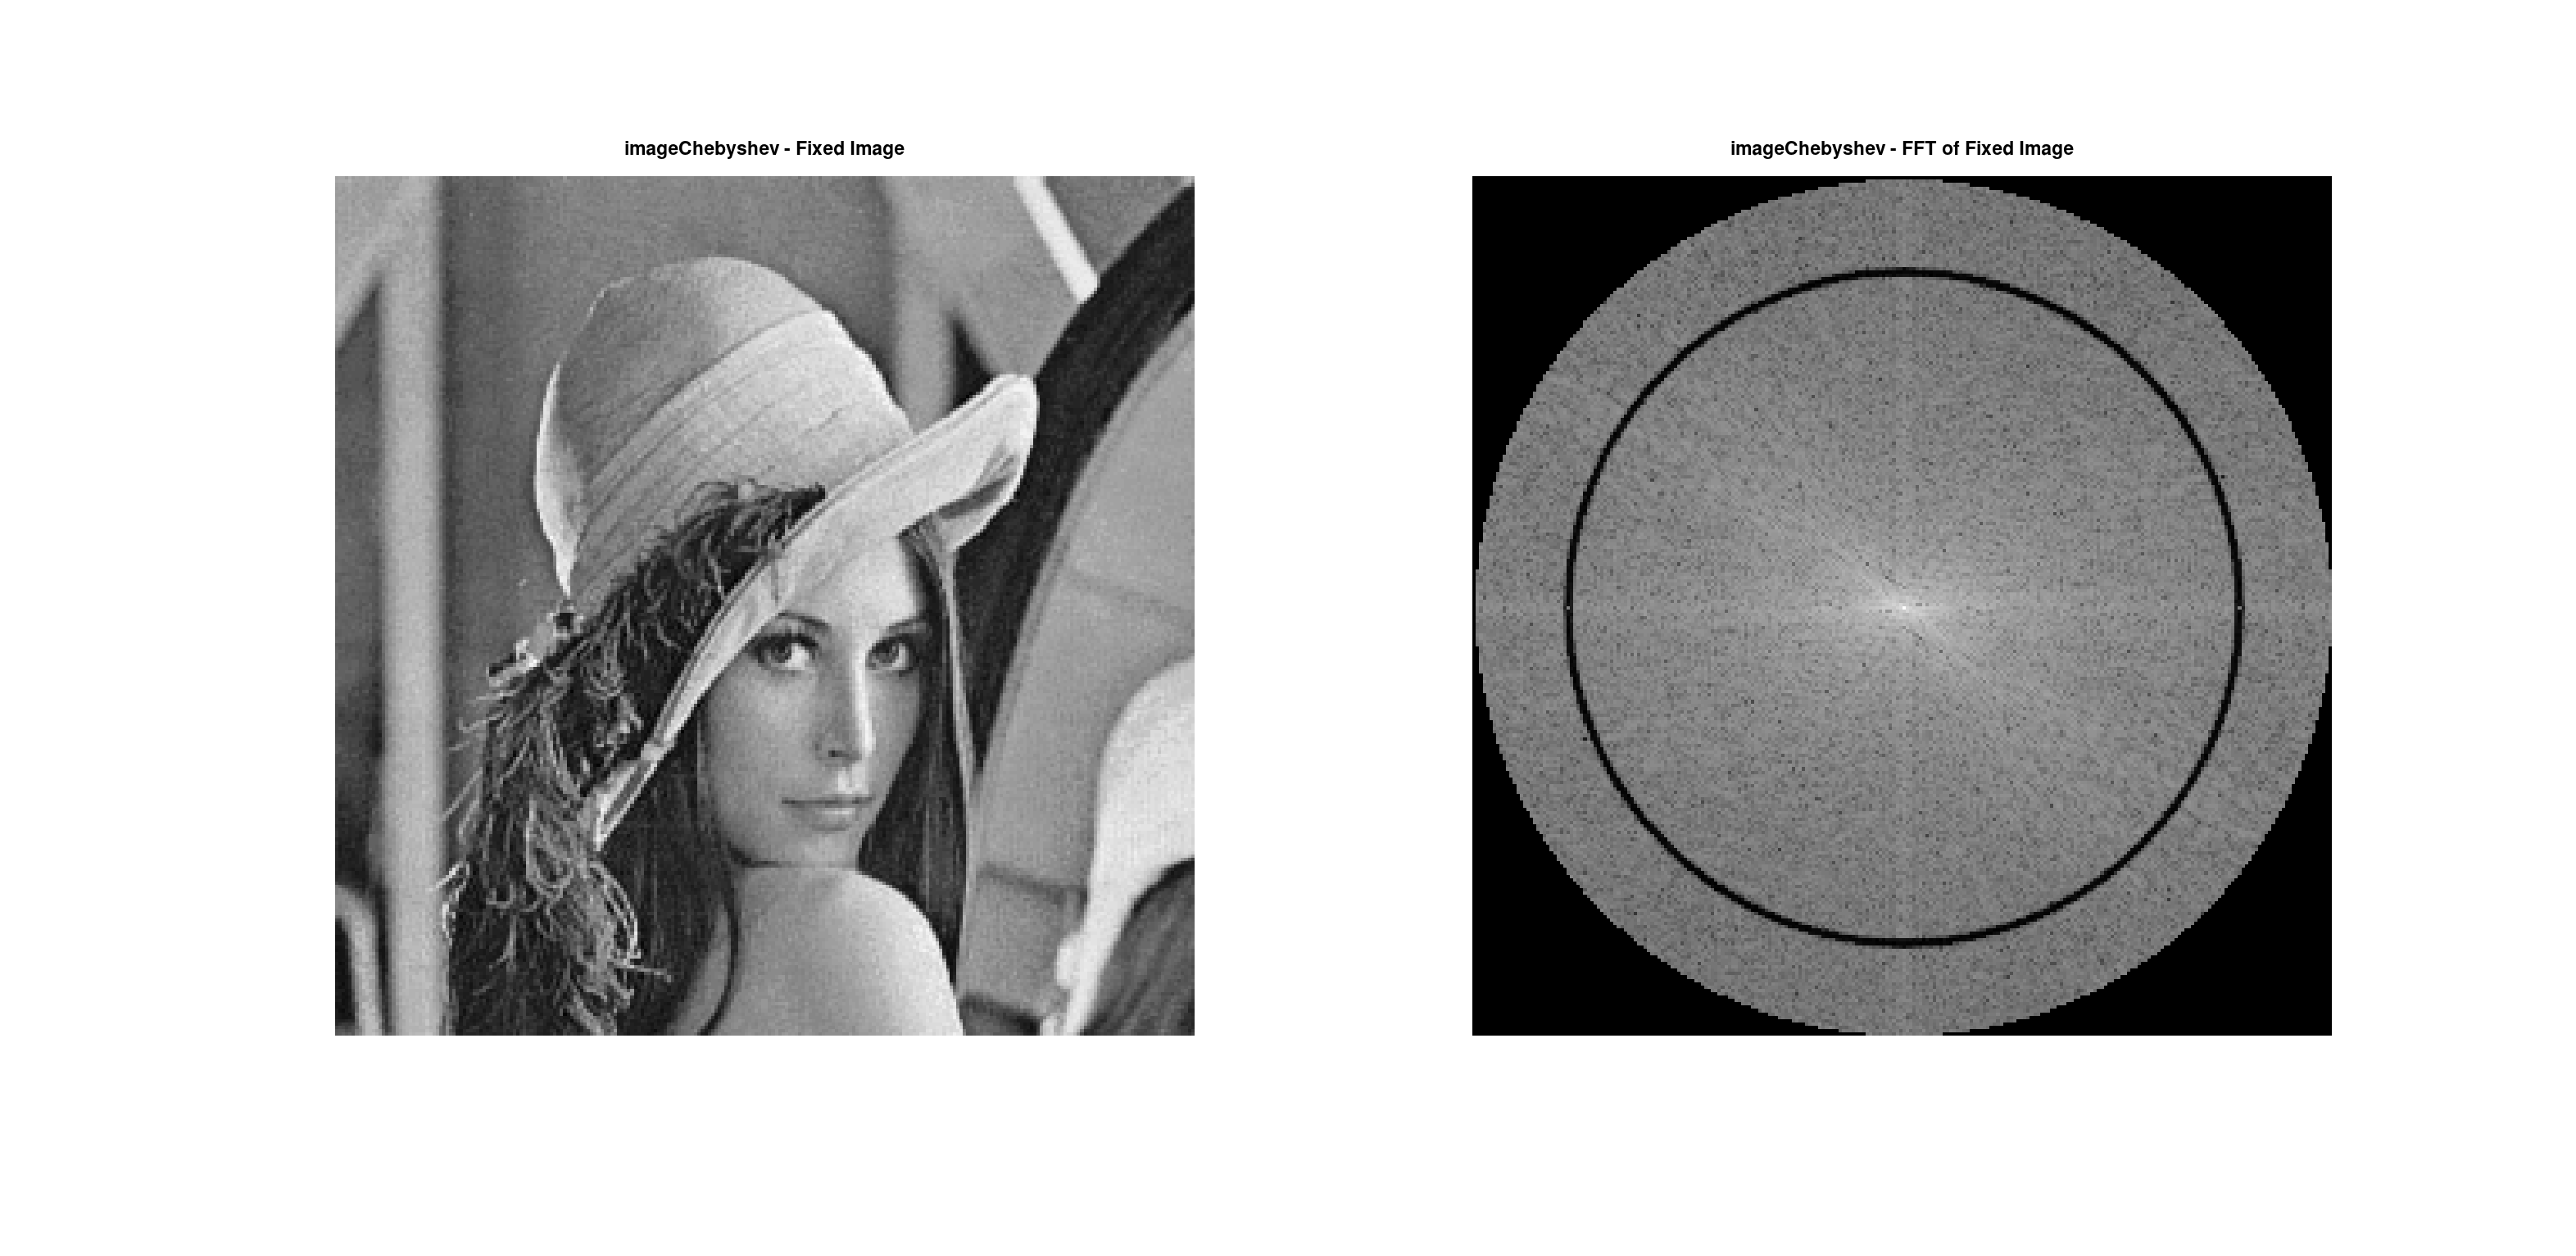
\includegraphics[width=1\linewidth]{03_results/assets/image_chebyshev.png}
    \caption{Imagem filtrada e seu espectro com o filtro Chebyshev.}
    \label{fig:image_chebyshev}
\end{figure}

Os filtros projetados, Butterworth e Chebyshev Tipo II, foram aplicados à imagem ruidosa com o objetivo de remover o ruído em uma faixa específica de frequências. Ambos os filtros utilizaram os mesmos parâmetros de banda passante e banda de rejeição, com uma largura de banda de rejeição de $1 \, \text{Hz}$ ($[99, 101] \, \text{Hz}$) e bandas passantes de $[98, 102] \, \text{Hz}$. Apesar das especificações iguais, as diferenças nas respostas dos filtros refletem as características únicas de suas arquiteturas.

No caso do filtro Butterworth, a ondulação máxima na banda passante foi limitada a $0.01 \, \text{dB}$ e a atenuação mínima na banda de rejeição foi de $20 \, \text{dB}$. Essas especificações resultaram em uma ordem de filtro de $n = 7$, evidenciando a necessidade de um maior número de coeficientes para lidar com as transições entre bandas em uma arquitetura conhecida pela suavidade de sua resposta.

Já o filtro Chebyshev Tipo II foi projetado com uma ondulação máxima de $1 \, \text{dB}$ na banda passante e uma atenuação mais rigorosa de $60 \, \text{dB}$ na banda de rejeição. Esse filtro também teve uma ordem de $n = 7$, o que, embora atípico para filtros Chebyshev Tipo II, é justificado pela alta exigência de atenuação e pela proximidade entre as bandas passante e de rejeição.

Embora o Chebyshev Tipo II geralmente exija uma ordem menor para atender às especificações, neste caso, a alta atenuação de $60 \, \text{dB}$ e a proximidade entre as bandas resultaram em uma ordem similar à do Butterworth. Ambos os filtros demonstraram eficácia na remoção do ruído, destacando-se por suas características individuais no processamento de imagens ruidosas.

\subsubsection*{Uso de filtros e seus parâmetros}

A partir da comparação entre os filtros aplicados no áudio e imagem, fica evidente que os filtros Elíptico e Chebyshev são mais eficientes em termos de atenuação, especialmente em aplicações que demandam uma rejeição acentuada de frequências indesejadas. Entretanto, essa maior eficiência vem acompanhada de uma maior instabilidade nas bandas de transição e na faixa passante, devido às oscilações características de suas respostas em frequência.

Por outro lado, o filtro Butterworth, embora menos performático em termos de rejeição, apresenta maior estabilidade e suavidade em suas bandas, sendo particularmente vantajoso em aplicações onde a preservação da integridade do sinal é crucial, como em áudio e imagens. Essa estabilidade torna o Butterworth uma escolha confiável quando se busca um compromisso entre filtragem eficaz e qualidade preservada.
